\id{ҒТАМР 50.43.00}{}

{\bfseries АДДИТИВТІ ӨНДІРІСТЕ CAD ЖӘНЕ CAE АҚПАРАТТЫҚ ТЕХНОЛОГИЯЛАРДЫ
ҚОЛДАНУ}

{\bfseries \textsuperscript{1}А.Тулегулов}
\begin{figure}[H]
	\centering
	
\includegraphics[width=0.8\textwidth]{media/ict2/image1}
	\caption*{}
\end{figure}
{\bfseries \textsuperscript{\envelope },
\textsuperscript{1}К.Акишев}

\begin{figure}[H]
	\centering
	
\includegraphics[width=0.8\textwidth]{media/ict2/image1}
	\caption*{}
\end{figure}
{\bfseries \textsuperscript{1}А.Джумагалиева}

\begin{figure}[H]
	\centering
	
\includegraphics[width=0.8\textwidth]{media/ict2/image1}
	\caption*{}
\end{figure}
{\bfseries ,\textsuperscript{2}И.Дюсебаев}

\begin{figure}[H]
	\centering
	
\includegraphics[width=0.8\textwidth]{media/ict2/image1}
	\caption*{}
\end{figure}


\textsuperscript{1}К. Құлажанов атындағы Қазақ технология және бизнес
университеті, Астана, Қазақстан,

\textsuperscript{2}Қ.И. Сәтбаев атындағы Қазақ ұлттық техникалық зерттеу
университеті, Алматы, Қазақстан

{\bfseries \textsuperscript{\envelope }}Корреспондент-автор:
\href{mailto:tad62@ya.ru}{\nolinkurl{tad62@ya.ru}}

Аддитивті өндіріс кәдімгі субтрактивті және деформацияланатын өндіріспен
салыстырғанда жоғары тұндыру жылдамдығымен күрделі 3D компоненттерін
жасауға мүмкіндік береді. Бірақ аддитивті өндіріс процесі әрқашан жылдам
қызумен және кейіннен салқындатумен бірге жүреді. Бұл өнімнің сапасына
кері әсер етуі мүмкін. Алайда аддитивті технологияның айқын
артықшылықтарына қарамастан процесті қатаң бақылауды қамтамасыз ету және
дайын өнімді алудың маңызды сәттері мен процедураларын автоматтандыру
қажет. Мақалада аддитивті өндірісте CAD және CAE компьютерлік
технологияларын қолдану қарастырылады.

Аддитивті өндіріс технологиясы-бұл материалдарды қабатты жинақтау арқылы
бөлшектерді өндіру технологиясы. Дәстүрлі технологиямен салыстырғанда
материалды жою (кесу), материалды жинақтаудың бұл әдісі кері тәртіпте
жүреді. Қосымша өндіріс технологиясы 1980 жылдардың аяғынан бастап
біртіндеп дамыды. Бұл технологияда материалдың жобалық деректері (соның
ішінде сұйықтықтар, ұнтақтар, сымдар немесе блоктар және т.б.) өндіріс
әдісін автоматты түрде қалыптастырады. Қосымша өндіріс технологиялары
дәстүрлі құралдарды, құрылғыларды және мультипроцессорлық процедураларды
қолдануды қажет етпейді.

3D дизайн деректерін пайдалана отырып, кез келген күрделі бөлшектерді
бір құрылғыда жылдам және дәл жасауға болады. Бұл технологиялық
процестер мен өңдеу циклін айтарлықтай азайтады. Өнімнің құрылымы
неғұрлым күрделі болса, оны жасаудың артықшылықтары соғұрлым маңызды
болады. Соңғы жылдары қосымша өндіріс технологиялары қарқынды дамуға қол
жеткізді. Қазіргі уақытта жабдықтың 20 дан астам түрі бар.

Бұл бағдарламалық жасақтаманың жоғары даму деңгейі олардың
қарапайымдылығымен және жұмыс процесінде қол жетімділігімен бірге оларды
күнделікті өндірістік тәжірибеде ақпараттық технологиялар саласында
терең білімі жоқ инженерлердің кең ауқымына қолдануға қосылуды
жеңілдетеді.

{\bfseries Түйін сөздер:} ақпараттық технологиялар, адаптивті жүйелер,
компьютерлік модель, автоматтандырылған дизайн, алгоритм.

{\bfseries ИСПОЛЬЗОВАНИЕ ИНФОРМАЦИОННЫХ ТЕХНОЛОГИЙ CAD И CAE В АДДИТИВНОМ
ПРОИЗВОДСТВЕ}

{\bfseries \textsuperscript{1}А. Тулегулов\textsuperscript{\envelope },
\textsuperscript{1}К. Акишев, \textsuperscript{1}Ж. Жантлесов,
\textsuperscript{1}М. Нурмагамбетов,}

{\bfseries \textsuperscript{1}А. Джумагалиева, \textsuperscript{2}И.
Дюсебаев}

\textsuperscript{1}Казахский университет технологии и бизнеса им.
Кулажанова, Астана, Казахстан,

\textsuperscript{2}Казахский национальный исследовательский технический
университет им. К. Сатпаева, Алматы, Казахстан,

e-mail: tad62@ya.ru

Аддитивное производство позволяет создавать сложные 3D-компоненты с
высокой скоростью осаждения по сравнению с обычным субтрактивным и
деформируемым производством. Но аддитивный производственный процесс
всегда сопровождается быстрым нагревом и последующим охлаждением. Это
может негативно сказаться на качестве продукта. Однако, несмотря на
очевидные преимущества аддитивной технологии, необходимо обеспечить
строгий контроль над процессом и автоматизировать основные моменты и
процедуры получения готового продукта.

Технология аддитивного производства-это технология производства деталей
путем многослойного накопления материалов. По сравнению с традиционной
технологией удаление материала (резка), этот метод накопления материала
происходит в обратном порядке. Технология дополнительного производства
постепенно развивалась с конца 1980-х годов. В этой технологии проектные
данные материала (включая жидкости, порошки, провода или блоки и т. д.)
автоматически формируют метод производства. Дополнительные технологии
производства не требуют использования традиционных инструментов,
устройств и многопроцессорных процедур.

Используя данные 3D-дизайна, вы можете быстро и точно создавать любые
сложные детали в одном устройстве. Это значительно сокращает
технологические процессы и цикл обработки. Чем сложнее структура
изделия, тем значительнее преимущества его изготовления. В последние
годы технологии дополнительного производства получили бурное развитие. В
настоящее время существует более 20 видов оборудования.

В статье рассматривается использование компьютерных технологий CAD и CAE
в аддитивном производстве. Высокий уровень разработки этого программного
обеспечения в сочетании с его простотой и доступностью в рабочем
процессе позволяет легко интегрировать их в применение широкому кругу
инженеров, не имеющих глубоких знаний в области информационных
технологий в повседневной производственной практике.

{\bfseries Ключевые слова:} информационные технологии, адаптивные системы,
компьютерная модель, автоматизированное проектирование, алгоритм.

{\bfseries THE USE OF CAD AND CAE INFORMATION TECHNOLOGIES IN ADDITIVE
MANUFACTURING}

{\bfseries \textsuperscript{1}A. Tulegulov\textsuperscript{\envelope },
\textsuperscript{1}K. Akishev, \textsuperscript{1}J. Zhantlesov,
\textsuperscript{1}M. Nurmagambetov,}

{\bfseries \textsuperscript{1}A. Dzhumagalieva, \textsuperscript{2}I.
Duisebaev}

\textsuperscript{1}Kazakh University of Technology and Business named
after Kulazhanova, Astana, Kazakhstan,

\textsuperscript{2}Kazakh National Research Technical University named
after K. Satpayev, Almaty, Kazakhstan,

e-mail: tad62@ya.ru

Additive production allows the creation of complex 3D components with a
high deposition rate compared to conventional subtractive and deformable
production. But the additive manufacturing process is always accompanied
by rapid heating and subsequent cooling. This can negatively affect the
quality of the product. However, despite the obvious advantages of
additive technology, it is necessary to ensure strict control over the
process and automate the most important points and procedures for
obtaining finished products. The article discusses the use of CAD and
CAE computer technologies in additive manufacturing.

Additive manufacturing technology is the technology of manufacturing
parts by layer accumulation of materials. Compared to traditional
technology material removal (cutting), this method of material
accumulation occurs in reverse order. Additional production technology
has developed gradually since the late 1980s. In this technology, the
design data of the material (including liquids, powders, wires or
blocks, etc.) automatically form the production method. Additional
production technologies do not require the use of traditional tools,
devices and multiprocessor procedures.

Using 3D design data, you can quickly and accurately create any complex
parts in one device. This significantly reduces the technological
processes and processing cycle. The more complex the structure of the
product, the more important the advantages of its manufacture. In recent
years, additional production technologies have achieved rapid
development. At the moment, there are more than 20 types of equipment.

The high level of development of these software, combined with their
simplicity and accessibility in the workflow, makes it easy to join them
in everyday production practice for a wide range of engineers who do not
have in-depth knowledge in the field of Information Technology.

{\bfseries Keywords:} information technologies, adaptive systems, computer
model, computer-aided design, algorithm.

{\bfseries Кіріспе.} Металды аддитивті өндіру (АӨ) - бұл автоматтандырылған
жобалау жүйесі (АЖЖ) деректерінің компьютерлік моделіне негізделген шикі
металды балқыту және оның қабатын қабат-қабат құру арқылы металл бөлігін
қабат-қабат жасайтын өндіріс технологиясы.

Соңғы бірнеше жылда бұл технология өнеркәсіптік қолдану үшін
пісіп-жетілді, негізінен жылдам өндірістің артықшылықтары,
материалдардың төмен құны және қолдануға болатын материалдардың кең
ауқымы. Мақсатқа байланысты аддитивті өндіріс технологиясының әртүрлі
түрлерін қолдануға болады. Мысалы, лазерлік және электронды сәулелер
жылу көзі ретінде пайдаланылады, ал ұнтақтар жоғары дәлдікті қажет
ететін ұсақ бөлшектер үшін шикізат ретінде пайдаланылады.

Ірі бөлшектер үшін қосымша катодты сәулелік өндіріс (EBAM) сияқты
балқыту әдістері қолданылады. Мысалы, титан сфералық резервуар
салыстырмалы түрде қарапайым. Катодты сәулелік балқыту вакуумдық
камерада жүзеге асырылады, бұл металдың тотығуын және кеуектердің пайда
болуын болдырмайды {[}1-2{]}

Аддитивті өндіріс кәдімгі субтрактивті және деформацияланатын өндіріспен
салыстырғанда жоғары тұндыру жылдамдығымен күрделі 3D компоненттерін
жасауға мүмкіндік береді. Бірақ аддитивті өндіріс процесі әрқашан жылдам
қызумен және кейіннен салқындатумен бірге жүреді. Бұл өнімнің сапасына
кері әсер етуі мүмкін.

Бұл мақалада 40x13 тот баспайтын болаттан жасалған бөлшектерді өндіруге
арналған шикізат ретінде жылу көзі және сым ретінде электронды сәулені
қолданатын аддитивті өндіріс технологиясы егжей-тегжейлі қарастырылады,
сонымен қатар бөлшектердің микроқұрылымы мен механикалық қасиеттері
талданады.

{\bfseries Әдеби шолу.} Аддитивті өндіріс технологиясы-бұл материалдарды
қабатты жинақтау арқылы бөлшектерді өндіру технологиясы. Дәстүрлі
технологиямен салыстырғанда материалды жою (кесу), материалды
жинақтаудың бұл әдісі кері тәртіпте жүреді. Қосымша өндіріс технологиясы
1980 жылдардың аяғынан бастап біртіндеп дамыды {[}3-4{]}. Бұл
технологияда материалдың жобалық деректері (соның ішінде сұйықтықтар,
ұнтақтар, сымдар немесе блоктар және т.б.) өндіріс әдісін автоматты
түрде қалыптастырады. Қосымша өндіріс технологиялары дәстүрлі
құралдарды, құрылғыларды және мультипроцессорлық процедураларды
қолдануды қажет етпейді.

3D дизайн деректерін пайдалана отырып, кез келген күрделі бөлшектерді
бір құрылғыда жылдам және дәл жасауға болады. Бұл технологиялық
процестер мен өңдеу циклін айтарлықтай азайтады. Өнімнің құрылымы
неғұрлым күрделі болса, оны жасаудың артықшылықтары соғұрлым маңызды
болады. Соңғы жылдары қосымша өндіріс технологиялары қарқынды дамуға қол
жеткізді. Қазіргі уақытта жабдықтың 20 дан астам түрі бар. {[}2{]}.

\emph{Лазерлік селективті балқыту}

Лазерлік селективті балқыту 1-суретте көрсетілген. Өнімді жасау процесі
ұнтақ түріне байланысты инертті газ аргон немесе азотпен толтырылған
машинаның SLM камерасында жүреді. Инертті газдың негізгі шығыны
вакуумдық камераны Үрлеу кезінде, одан ауа толығымен шығарылған кезде
пайда болады (оттегінің рұқсат етілген мөлшері 0,15\% - дан аз). Осыдан
кейін өнім пластинамен бірге SLM машинасының камерасынан шығарылады,
содан кейін өнім пештен механикалық түрде бөлінеді. Әрі қарай, салынған
өнімді әрлеу жұмыстары жүреді. Оттегінің толық болмауы титан сияқты
материалдармен жұмыс істеуге мүмкіндік беретін шығын материалының
тотығуын болдырмайды {[}5-6{]}.


\begin{figure}[H]
	\centering
	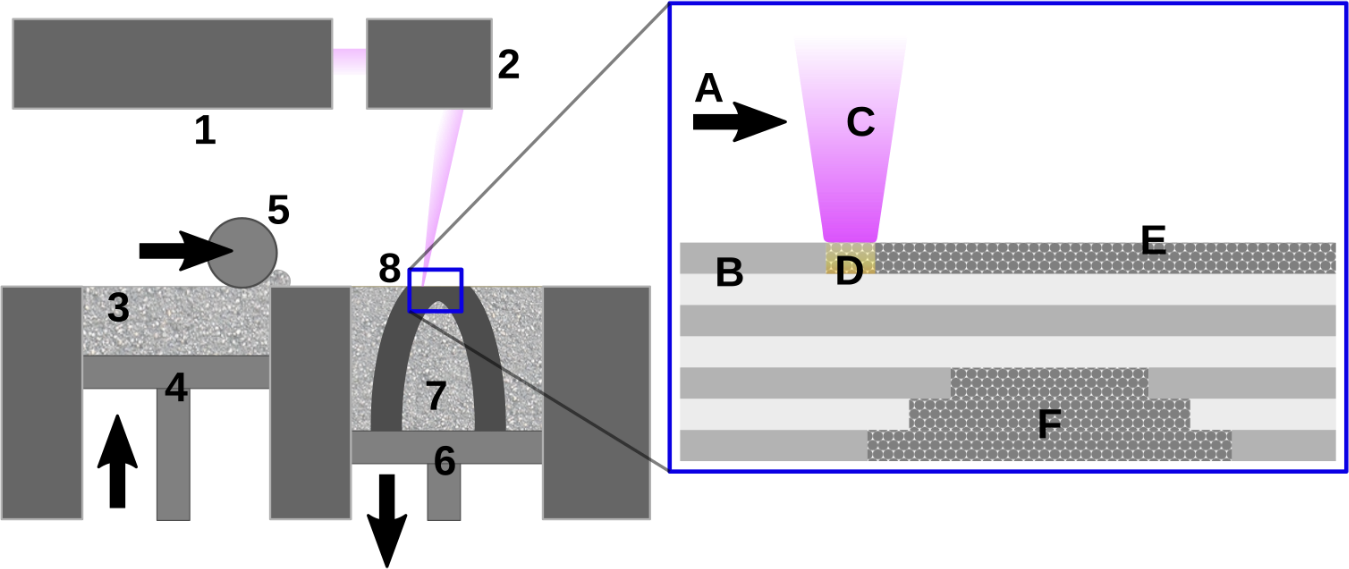
\includegraphics[width=0.8\textwidth]{media/ict2/image187}
	\caption*{}
\end{figure}


{\bfseries 1 - сурет. Лазерлік селективті балқыту}

Лазерлік балқыту (SLM) - дайындау технологиясы көмегімен күрделі
кеңістіктік пішіндегі металл бұйымдарын ұнтақ құрамдарын лазермен
балқыту. Жұмыстар математикалық модель негізінде орындалады. Металл
ұнтақтарының тез балқуын қамтамасыз ету үшін SLM технологиясы
қолданылады. Қазіргі уақытта жоғары энергия тығыздығы бар лазерлерді
қолданады. Жылу көзі ретінде қуаты 50-400 Вт және дақ мөлшері 20-100 мкм
болатын лазер қолданылады. Бұл іс жүзінде бөлшектерді тікелей алуға
мүмкіндік береді {[}7-8{]}. Алынған бөлшектерде пішіні ұсақ түйіршікті,
біртекті құрылым, бетінің кедір-бұдырлығы 20-50 мкм жетуі мүмкін. Бұл
әртүрлі дайындамаларды өңдеуге жарамды технологияның күрделі түрі. SLM
жоғары дәлдікке ие болғанымен, ол қалыптау процесінде сфероидизация
құбылысына тап болады {[}9-10{]}

{\bfseries Материалдар мен әдістер.} Эксперименттерде шикізат ретінде сым
қолданылды

диаметрі 1,2 мм 40Х13 маркалы легирленген тот баспайтын болаттан
жасалған. Субстраттың өлшемдері 100×100×19 ММ. негізгі субстрат тірек
тақтасына орналастырылған және қысқыштармен мықтап басылған.
Мүмкіндігінше қысуды қамтамасыз ету үшін субстраттың бұрыштарына екі
қысқыш орналастырылған. Негізгі субстрат балқытылған шикізатты қолдану
арқылы тікелей қолданылады.(1 кесте)

{\bfseries 1 кесте - 40x13 тот баспайтын болаттан жасалған сым}

%% \begin{longtable}[]{@{}
%%   >{\centering\arraybackslash}p{(\linewidth - 18\tabcolsep) * \real{0.1773}}
%%   >{\centering\arraybackslash}p{(\linewidth - 18\tabcolsep) * \real{0.0814}}
%%   >{\centering\arraybackslash}p{(\linewidth - 18\tabcolsep) * \real{0.0805}}
%%   >{\centering\arraybackslash}p{(\linewidth - 18\tabcolsep) * \real{0.0806}}
%%   >{\centering\arraybackslash}p{(\linewidth - 18\tabcolsep) * \real{0.0968}}
%%   >{\centering\arraybackslash}p{(\linewidth - 18\tabcolsep) * \real{0.0890}}
%%   >{\centering\arraybackslash}p{(\linewidth - 18\tabcolsep) * \real{0.1019}}
%%   >{\centering\arraybackslash}p{(\linewidth - 18\tabcolsep) * \real{0.0830}}
%%   >{\centering\arraybackslash}p{(\linewidth - 18\tabcolsep) * \real{0.0968}}
%%   >{\centering\arraybackslash}p{(\linewidth - 18\tabcolsep) * \real{0.1128}}@{}}
%% \toprule\noalign{}
%% \begin{minipage}[b]{\linewidth}\centering
%% Элемент
%% \end{minipage} & \begin{minipage}[b]{\linewidth}\centering
%% С
%% \end{minipage} & \begin{minipage}[b]{\linewidth}\centering
%% Si
%% \end{minipage} & \begin{minipage}[b]{\linewidth}\centering
%% Mn
%% \end{minipage} & \begin{minipage}[b]{\linewidth}\centering
%% Cr
%% \end{minipage} & \begin{minipage}[b]{\linewidth}\centering
%% S
%% \end{minipage} & \begin{minipage}[b]{\linewidth}\centering
%% P
%% \end{minipage} & \begin{minipage}[b]{\linewidth}\centering
%% Ti
%% \end{minipage} & \begin{minipage}[b]{\linewidth}\centering
%% Cu
%% \end{minipage} & \begin{minipage}[b]{\linewidth}\centering
%% Ni
%% \end{minipage} \\
%% \midrule\noalign{}
%% \endhead
%% \bottomrule\noalign{}
%% \endlastfoot
%% \% & 0.36- & ≤0.8 & ≤0.8 & 12.0- & ≤0.03 & ≤0.025 ≤0.2 & ≤0.3 & ≤0.6 &
%% 0.36- \\
%% \end{longtable}

Субстраттың қозғалыс механизмі 2 суретте көрсетілген.


\begin{figure}[H]
	\centering
	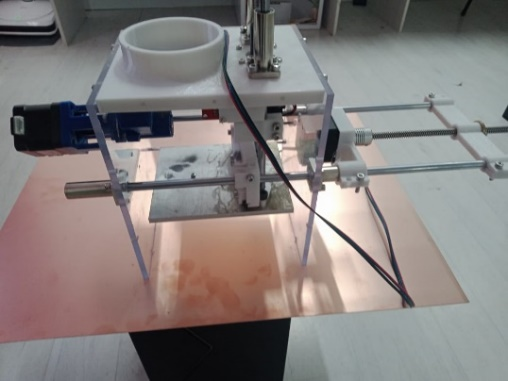
\includegraphics[width=0.8\textwidth]{media/ict2/image188}
	\caption*{}
\end{figure}


{\bfseries 1 - сурет. Субстраттың қозғалыс механизмі}

Басып шығару механизмі 3-суретте көрсетілген.


\begin{figure}[H]
	\centering
	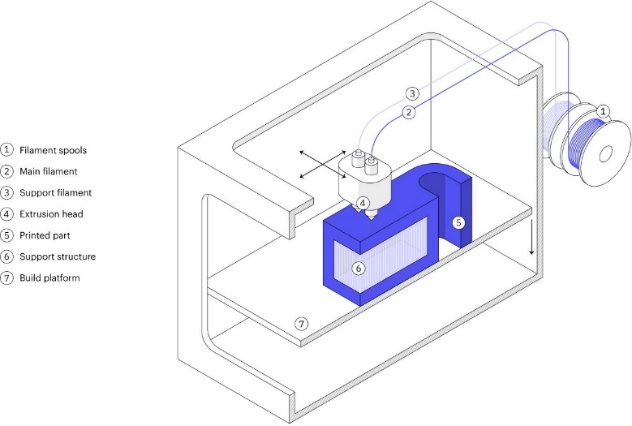
\includegraphics[width=0.8\textwidth]{media/ict2/image189}
	\caption*{}
\end{figure}


{\bfseries 3 - сурет. Басып шығару механизмі}

{\bfseries Нәтижелер мен талқылау.} Бұл зерттеу үш түрлі эксперименттің
нәтижелерін ұсынады. Бірнеше эксперименттерден кейін ток күшінің оңтайлы
мәні анықталды.4-суретте токтың номиналды мәні бойынша алынған үлгінің
фрагменті (а үлгісі) көрсетілген.


\begin{figure}[H]
	\centering
	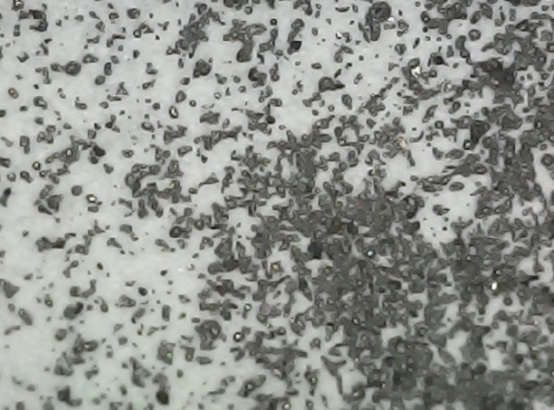
\includegraphics[width=0.8\textwidth]{media/ict2/image190}
	\caption*{}
\end{figure}


{\bfseries 4 - сурет. Токтың номиналды мәні бойынша алынған үлгінің
үзіндісі}

Жоғары ток кезінде дәнекерлеудің артық балқуы анықталды. Бірінші қабатта
ең жоғары салқындату жылдамдығы бар. Эксперимент процесінде бөлшек
белгілі бір биіктікке жеткенде, оның жылдамдығы байқалады салқындату
азаяды, нәтижесінде сым төмендейді сұйық металл күйі және дайындаманың
айналасында қозғалады (2 кесте)

\emph{Үлгі А}

{\bfseries 2-кесте. А үлгісін басып шығару параметрлері}

%% \begin{longtable}[]{@{}
%%   >{\raggedright\arraybackslash}p{(\linewidth - 2\tabcolsep) * \real{0.4394}}
%%   >{\raggedright\arraybackslash}p{(\linewidth - 2\tabcolsep) * \real{0.5606}}@{}}
%% \toprule\noalign{}
%% \begin{minipage}[b]{\linewidth}\raggedright
%% Сым диаметрі: 1,2 мм
%% \end{minipage} & \begin{minipage}[b]{\linewidth}\raggedright
%% Сәулелік шеңбер: 3-5мм
%% \end{minipage} \\
%% \midrule\noalign{}
%% \endhead
%% \bottomrule\noalign{}
%% \endlastfoot
%% Үдеткіш кернеу: 400 В & Сым беру бұрышы: 45° \\
%% Сәулелік Ток: 21ма & Электронды сәуленің тиімділігі: 0.85-0.95 \\
%% Қабаттың қалыңдығы: 0, 877мм & Қабат саны: 100 \\
%% \multicolumn{2}{@{}>{\raggedright\arraybackslash}p{(\linewidth - 2\tabcolsep) * \real{1.0000} + 2\tabcolsep}@{}}{%
%% ұзындығы: 21мм ені: 21мм биіктігі: 76мм (шамамен) субстратты біртіндеп
%% қыздыру температура-Жоқ, жоғары қуатпен(+5-10мА) бірінші қабатта} \\
%% \multicolumn{2}{@{}>{\raggedright\arraybackslash}p{(\linewidth - 2\tabcolsep) * \real{1.0000} + 2\tabcolsep}@{}}{%
%% Жылдамдық сканерлеу (5-сурет) сым беру (6-сурет)
%% 
%% Қалыптасу жылдамдығы (м\textsuperscript{3}/сағ) 6.9×10\^{}-5 бір қабат
%% үшін уақыт 20.8 s} \\
%% \end{longtable}


\begin{figure}[H]
	\centering
	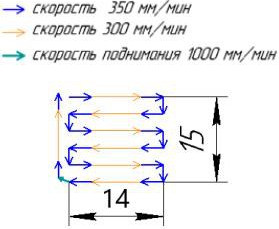
\includegraphics[width=0.8\textwidth]{media/ict2/image191}
	\caption*{}
\end{figure}


{\bfseries 5 - сурет. Басып шығару жылдамдығының диаграммасы}


\begin{figure}[H]
	\centering
	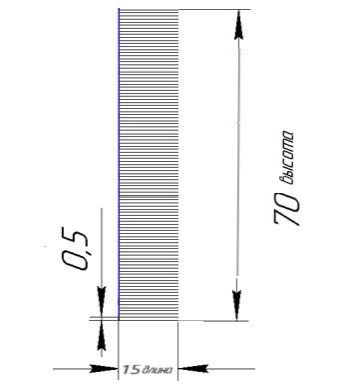
\includegraphics[width=0.8\textwidth]{media/ict2/image192}
	\caption*{}
\end{figure}


{\bfseries 6 - сурет. Басып шығару траекториясының схемасы}

Дәстүрлі өндіріс әдістерінен айырмашылығы, олар мартенситті тот
баспайтын болаттар әдетте толығымен мартенситті болып табылады, аустенит
және Дельта феррит фазалары сияқты басқа микроскопиялық компоненттерді
аддитивті түрде жасалған мартенситті тот баспайтын болаттардан табуға
болады.

7 суретте көрсетілгендей, микроқұрылымдық сипаттама 40x13 тот баспайтын
болаттан жасалған басылған үлгі жарықтар пайда болмай, толығымен тығыз
құрылым екенін көрсетеді. Балқытылған ваннаның шекарасы жоқ, бұл
материалдың басып шығару процесінде жақсы балқығанын көрсетеді.
Микроқұрылым мартенсит пен аустениттен тұрады, тесіктері мен қоспалары
жоқ.

а в с

{\bfseries 6 - сурет. А-21ma металлографиялық микроскопының астындағы
Микроқұрылым; B-31mA; С-33 ma}

Қазіргі заманғы бағдарламалық жасақтама, көп жағдайда, CAE жүйелерін
қолдана отырып, компьютерлік модельдеу саласына бәрін аудара отырып,
табиғи эксперименттен толық немесе ішінара бас тартуға мүмкіндік береді.
CAD жүйелерін қолдану арқылы неғұрлым көп жұмыс жасалса және жаңа
өнімдердің үш өлшемді графикалық модельдері неғұрлым көп жасалса,
компьютерлік талдауды қолдану соғұрлым қызықты болады.

Сонымен қатар, CAD және CAE жүйелерін жақындастыру өте қиын. Графикалық
және есептік модельдер айтарлықтай ерекшеленетінін талап ете отырып,
соңғысының әзірлеушілері көбінесе CAE бағдарламасына енгізілген
редакторларды қолдана отырып, есептік модельдерді нөлден әзірлеудің
орындылығын талап етеді.

{\bfseries Қорытынды.} Микроқұрылымдық талдау 40Х13 өлшемді баспайтын
болаттан жасалған басылған үлгі толығымен тығыз, жарықсыз құрылым екенін
көрсетеді. Балқытылған ваннаның шекаралары жоқ, бұл сым материалы басып
шығару процесінде ерігенін көрсетеді. Микроқұрылым ине тәрізді мартенсит
пен қалдық аустениттен тұрады, тесіктері мен қоспалары жоқ\emph{.}

\emph{{\bfseries Қаржыландыру:}Бұл зерттеуді ғылым және жоғары білім
комитеті қаржыландырады (№АР23490424 "Қорғаныс өнеркәсібі үшін металл
нысандарын жасау үшін аддитивті қондырғыны әзірлеу".)}

{\bfseries Әдебиеттер}

1. Тулегулов А.Д., Юрков Н.К. Аддитивные технологии для создания
металлических объектов для военной техники и вооружения. Вестник
Академии национальной гвардии Республики Казахстан. - 2024. - № 3(53). -
С.151-157.

2. Akishev K., Nurtai Zh., Akisheva L. Akisheva. Automation of selection
of construction mix with additives of technogenic raw materials //
Vestnik KazUTB. - 2025. - Vol.1 (26). - 2025. - P.1-14. DOI
10.58805/kazutb.v.1.26-808.

3. Акишев К.М., Жамангарин Д.С., А. Талғат. Басқару алгоритмі бар
микроконтроллер арқылы негізделген энергиясы есепке алудық
интеллектуалды жүйсе. Военный научно-технический журнал
военно-инженерного института радиоэлектроники и связи. -- 2022. - №
4(50). - С.136 -143.

4. Бородин, И.Ф., Андреев С.А. Автоматизация технологических процессов и
системы автоматического управления (ССУЗ) / Колосс. - 2006. - 352 c.
ISBN: 5-9532-0140-0.

5. Брюханов, В.Н. Автоматизация производства /Высшая школа. - 2016. -
367 c. ISBN 5-06-004453-X: 3000

6. Клюев, А.С. Автоматизация настройки систем управления / Альянс. -
2015. - 272 c.

7. Каменев, С. В. Технологии аддитивного производства: учебное пособие
для СПО / Профобразование. - 2020. - 144 c. ISBN 978-5-4488-0564-6.

8. Ляпков А.А. Современные аддитивные технологии: учебное пособие /
КноРус. - 2024. - 234 с. ISBN 978-5-406-12661-5

9. Ford S. Additive Manufacturing Technology: Potential Implications for
U.S. Manufacturing Competitiveness // Journal of International Commerce
and Economics. Published electronically. - 2014.
URL:~\url{https://ssrn.com/abstract=2501065}. -Date of address:
18.01.2025

10. Stephen L. A Fully Functional 3-D Printed Heart Sooner Than You
Think // Qmed. - 2014. URL:
\url{http://www.qmed.com/mpmn/medtechpulse/fully-functional-3-d-printed-heartsooner-you-think}.
Date of address: 18.01.2025

{\bfseries References}

1. Tulegulov A.D., Jurkov N.K. Additivnye tehnologii dlja sozdanija
metallicheskih ob\#ektov dlja voennoj tehniki i vooruzhenija. Vestnik
Akademii nacional' noj gvardii Respubliki Kazahstan. -
2024. - № 3(53). - S.151-157.{[}in Russian{]}

2. Akishev K., Nurtai Zh., Akisheva L. Akisheva. Automation of selection
of construction mix with additives of technogenic raw materials //
Vestnik KazUTB. - 2025. - Vol.1 (26). - 2025. - P.1-14. DOI
10.58805/kazutb.v.1.26-808. {[}in Russian{]}

3. Akishev K.M., Zhamangarin D.S., A. Talғat. Basқaru algoritmі bar
mikrokontroller arқyly negіzdelgen jenergijasy esepke aludyқ
intellektualdy zhүjse. Voennyj nauchno-tehnicheskij zhurnal
voenno-inzhenernogo instituta radiojelektroniki i svjazi. -- 2022. - №
4(50). - S.136 -143. {[}in Russian{]}

4. Borodin, I.F., Andreev S.A. Avtomatizacija tehnologicheskih processov
i sistemy avtomaticheskogo upravlenija (SSUZ) / Koloss. - 2006. - 352 c.
ISBN: 5-9532-0140-0. {[}in Russian{]}

5. Brjuhanov, V.N. Avtomatizacija proizvodstva /Vysshaja shkola. - 2016.
- 367 c. ISBN 5-06-004453-X: 3000. {[}in Russian{]}

6. Kljuev, A.S. Avtomatizacija nastrojki sistem upravlenija /
Al' jans. - 2015. - 272 c.

7. Kamenev, S. V. Tehnologii additivnogo proizvodstva: uchebnoe posobie
dlja SPO / Profobrazovanie. - 2020. - 144 c. ISBN 978-5-4488-0564-6.
{[}in Russian{]}

8. Ljapkov A.A. Sovremennye additivnye tehnologii: uchebnoe posobie /
KnoRus. - 2024. - 234 s. ISBN 978-5-406-12661-5. {[}in Russian{]}

9. Ford S. Additive Manufacturing Technology: Potential Implications for
U.S. Manufacturing Competitiveness // Journal of International Commerce
and Economics. Published electronically. - 2014.
URL:~\url{https://ssrn.com/abstract=2501065}. -Date of address:
18.01.2025

10. Stephen L. A Fully Functional 3-D Printed Heart Sooner Than You
Think // Qmed. - 2014. URL:
\url{http://www.qmed.com/mpmn/medtechpulse/fully-functional-3-d-printed-heartsooner-you-think}.
Date of address: 18.01.2025

\emph{{\bfseries Авторлар туралы мәліметтер}}

Тулегулов А.Д.- физика-математика ғылымдарының кандидаты,
қауымдастырылған профессор, Қ. Құлажанов атындағы ҚазТБУ, Астана,
Қазақстан, e-mail: \href{mailto:tad62@ya.ru}{\nolinkurl{tad62@ya.ru}};

Акишев К.М.- -техника ғылымдарының кандидаты, қауымдастырылған
профессор, Қ. Құлажанов атындағы ҚазТБУ, Астана, Қазақстан, e-mail:
akmail04@mail.ru;

Жұмағалиева А.М.- магистр, қауымдастырылған профессор, Қ. Құлажанов
атындағы ҚазТБУ, Астана, Қазақстан, e-mail:
\href{mailto:Dzhum@mail.ru}{\nolinkurl{Dzhum@mail.ru}};

Дюсебаев І.- PhD докторы, Қ. Сәтбаев атындағы Қазақ ұлттық зерттеу
университеті, Алматы, Қазақстан, e-mail:
\href{mailto:Nomad13@mail.ru}{\nolinkurl{Nomad13@mail.ru}}.

\emph{{\bfseries Information about the authors}}

Tulegulov A.D. - Candidate of Physical and Mathematical Sciences,
Associate Professor, K. Kulazhanov KazUTB, Astana, Kazakhstan, e-mail:
tad62@ya.ru;

Akishev K.A. - Candidate of Technical Sciences, Associate Professor, K.
Kulazhanov KazUTB, Astana, Kazakhstan, e-mail: akmail04@mail.ru;

3. Dzhumagalieva A.M.- Master, Associate Professor, K. Kulazhanov
KazUTB, Astana, Kazakhstan, e-mail: Dzhum@mail.ru;

Dyusebayev I. - Dr. PhD, K.I. Satpayev Kazakh National Research
University, Almaty, Kazakhstan, e-mail: Nomad.i.m.13@mail.ru.\